\documentclass[12pt]{article}
\usepackage{geometry,fancyhdr,xr,hyperref,ifpdf,amsmath,rcs,shortcuts}
\usepackage{lastpage,longtable,color,paunits,amsmath,smallsec}
\geometry{letterpaper,top=50pt,hmargin={20mm,20mm},headheight=15pt} 


\pagestyle{fancy} 

\RCS $Revision: 1.5 $
\RCS $Date: 2002/01/09 03:50:54 $

\fancypagestyle{first}{
\lhead{Diffusion notes}
\chead{}
\rhead{page~\thepage/\pageref{LastPage}}
\lfoot{} 
\cfoot{} 
\rfoot{}
}

\ifpdf
    \usepackage[pdftex]{graphicx} 
    \usepackage{hyperref}
    \pdfcompresslevel=0
    \DeclareGraphicsExtensions{.pdf,.jpg,.mps,.png}
\else
    \usepackage{hyperref}
    \usepackage[dvips]{graphicx}
    \DeclareGraphicsRule{.eps.gz}{eps}{.eps.bb}{`gzip -d #1}
    \DeclareGraphicsExtensions{.eps,.eps.gz}
\fi
\externaldocument[lec6,]{lec6}

\begin{document}
\newcommand{\vect}[1]{\boldsymbol{\vec{#1}}}
\pagestyle{first}

\begin{center}
Atsc405: Crystal growth via diffusion\\
\end{center}


\section{Introduction}
\label{sec:introduction}

The crystal growth equation (Lohmann equation 8.11 and problem 4) uses the crystal capacitance C.
Below we look at where that comes from.

Recall from the droplet growth notes that we used
spherical symmetry to derive this  equation

\begin{equation}
  \label{eq:diff}
  \frac{ dm}{dt} = 4 \pi x^2 D \frac{ d\rho_v}{dx} 
\end{equation}
where $m$ is the droplet mass, $x$ is the radial coordinate
in a spherical coordinate system and $D \frac{ d\rho_v}{dx} $ is the
diffusive flux of water vapor through radius x in the direction
of the drop center.  When we integrate this twice we get:

\begin{gather}
  \label{final}
  \frac{dr}{dt} = \frac{ D}{r\rho_l}  (\rho_{v \infty} - \rho_{v}(r) )
\end{gather}



This is the equivalent  equation for crystals:


\begin{gather}
  \label{finalC}
  \frac{dm}{dt} = \frac{ D C}{\epsilon_0}  \left ( \rho_{v \infty} - \rho_{vc}  \right )
\end{gather}
where $m$ is the mass of the crystal, $C$ is the capcitance (in Farads) and 
$\epsilon_0$ is the permittivity of free space (in Farads/meter).
What are these electrostatic constants doing in an equation about vapor growth?


\section{Derivation}
\label{sec:mass-continuity}

Remember Fick's law:


\begin{equation}
  \label{eq:vaporflux}
\frac{ dm}{dt} = F_{vapor} = - \oint D \nabla   \rho_v ds
\end{equation}
where the integral is taken over the surface of the crystal, and by definition
the flux through the surface is contributing to the crystal growth
rate $dm/dt$.


Compare (\ref{eq:vaporflux}) to Gauss' law for the relationship
between the charge on a capacitor Q (Coulombs) and
the voltage $\phi$.

\begin{equation}
  \label{eq:coloumb}
\frac{ Q}{\epsilon_0}  = - \oint  \nabla   \phi ds
\end{equation}

If we make a ice crystal out of copper and place it inside
a conducting enclosure we have a capacitor.  We can relate
the charge stored in the capacitor to the voltage on the
conductor ($\phi_\infty$) and the copper crystal $\phi_c$
through the capcitance, $C$:

\begin{equation}
  \label{eq:cap}
  Q = C ( \phi_\infty - \phi_c )
\end{equation}

To use this, let's relate $\phi$ and $\rho$ through
an arbitrary constant $\beta$ (which will divide out):

\begin{equation}
  \label{eq:beta}
  \rho_v = \beta \phi
\end{equation}

then

\begin{equation}
  \label{eq:cap2}
  Q = C ( \frac{\rho_\infty}{\beta}  - \frac{\rho_c}{\beta} )
\end{equation}
and 

\begin{equation}
  \label{eq:coloumb2}
\frac{ Q}{\epsilon_0}  = - \oint \frac{1}{\beta} \nabla \rho   ds
\end{equation}
Substitute for $Q$ between (\ref{eq:cap2}) and (\ref{eq:coloumb2}):

\begin{equation}
  \label{eq:coloumb3}
- \epsilon_0 \oint \frac{1}{\beta} \nabla \rho   ds = C ( \frac{\rho_\infty}{\beta}  - \frac{\rho_c}{\beta} )
\end{equation}
and clear the $\beta$ and $\epsilon$ and plug (\ref{eq:coloumb3}) into (\ref{eq:vaporflux}):

\begin{equation}
  \label{eq:vaporflux2}
\frac{ dm}{dt} =  - \oint D \nabla   \rho_v ds =
\frac{D C }{\epsilon_0} \left ( \rho_\infty - \rho_c \right )
\end{equation}

Note that the units work:  


\begin{equation}
  \label{eq:units}
D\ (\un{m^2\,s^{-1}}) \times C\ (\un{Farads}) \times \frac{ 1}{\epsilon_0}
\ ( \un{m\,Farad^{-1}} ) \times \rho \ (\un{kg\,m^{-3}} ) = \un{kg\,s^{-1}}
\end{equation}


and here are some capacitances:

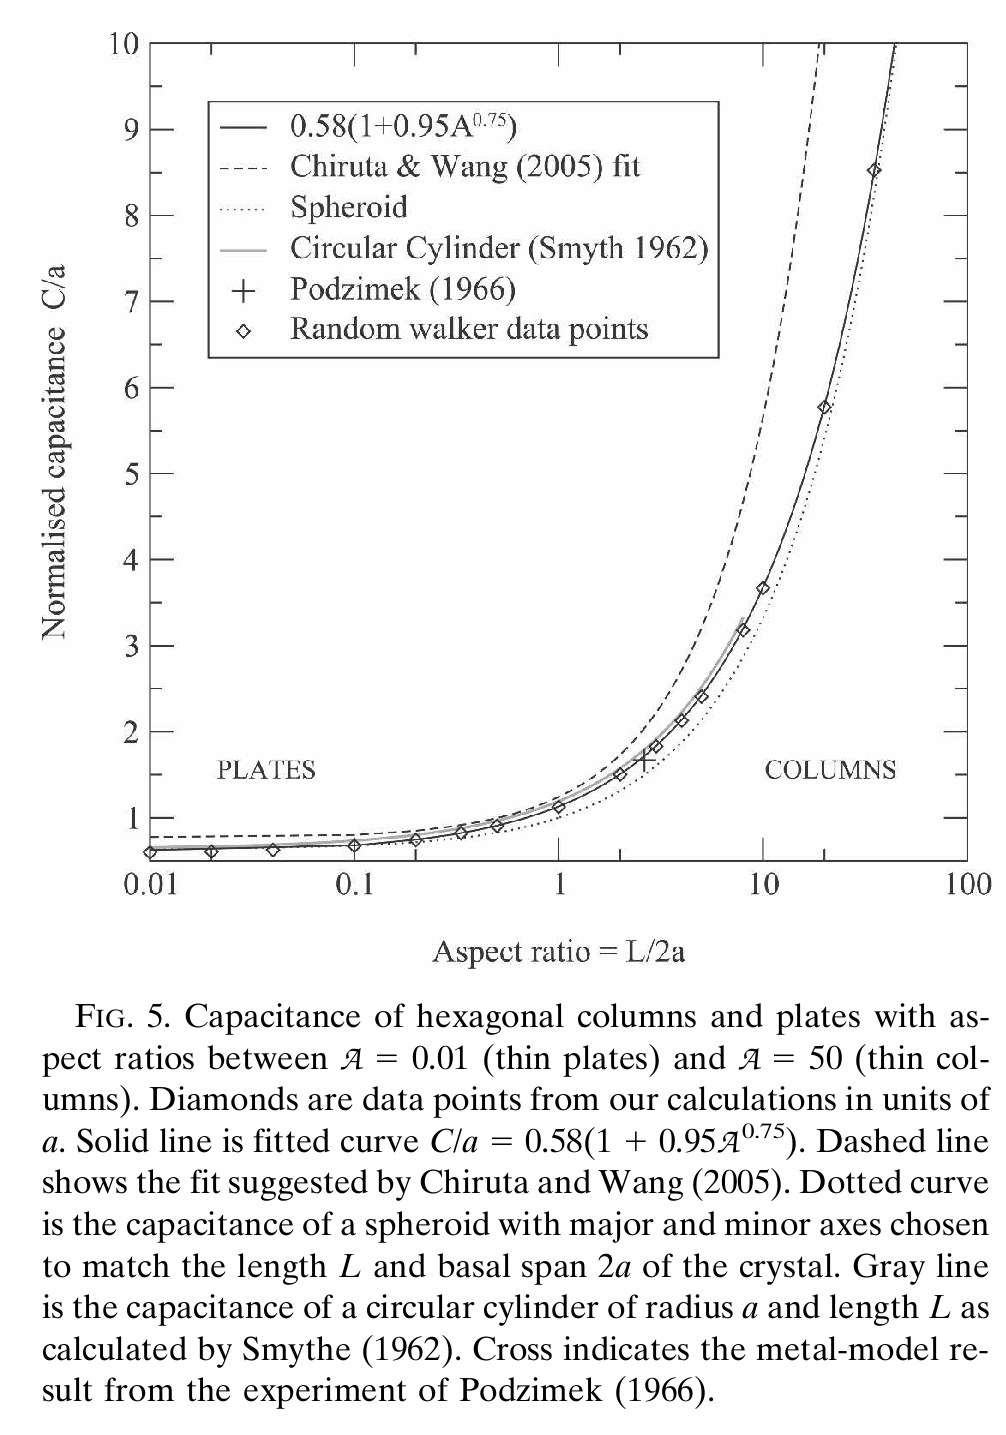
\includegraphics[width=0.6\textwidth]{capacitance.png}


\end{document}
%%% Local Variables:
%%% mode: latex
%%% TeX-master: t
%%% End:
